\section{Taxonomy}
\label{sec:taxonomy}

Traditionally, fingerprinting methods are classified into active and passive based on interaction with the target system \cite{spitzner}. Active fingerprinting involves the creation of specific probes and using them to query the target system to collect as much data possible. On the contrary, passive fingerprinting makes use of available metadata and analysis to determine information about the target. Passive fingerprinting limits communication with the target system as much as possible. Remote attackers tend to use active fingerprinting methods more because passive approaches do not lead to an inference. This is because passive fingerprinting requires detailed analysis of collected meta data. Passive fingerprinting techniques also depend on fingerprint databases to infer their findings. Fingerprint databases contain information about distinct responses by systems on interaction.
   
Based on the honeypot fingerprinting techniques summarized in Section \ref{sec:hft}, we propose a taxonomy based on the detection methods employed by these techniques. We classify the techniques under Probe based approach, Metadata based approach and \acrlong{ml} based approach. Figure \ref{fig:taxonomy} provides an overview of the classified techniques on the proposed taxonomy.We summarize each of the detection methods in the below sub sections. 

\begin{figure}[t]
    \centering
    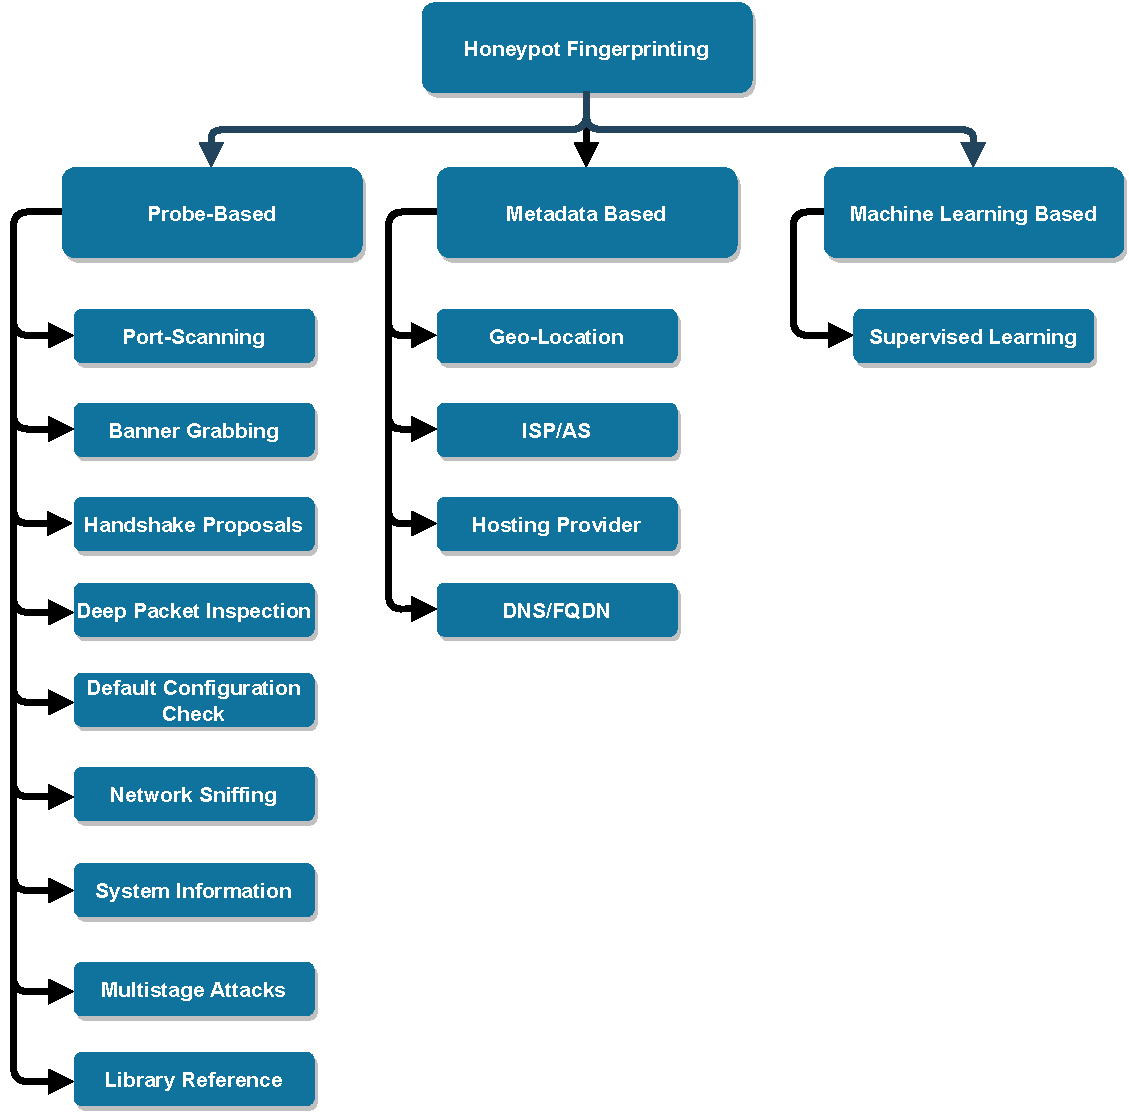
\includegraphics[scale=0.45]{taxo}
    \caption{Honeypot Fingerprinting Taxonomy}
    \label{fig:taxonomy}
\end{figure}

\subsection{Probe-based fingerprinting}
\label{Probe Based}
Probe-based fingerprinting involves the creation of crafted queries to target devices to derive fingerprinting information. The techniques classified under this methods require the need to interact with the target system to retrieve fingerprinting information. The probe-based methods engage with the target system, unlike the metadata methods. These methods focus on leveraging the responses from communication protocols and classifying the target machine based on specific values from the responses. Constructing probes is an advanced method that requires proficient knowledge of systems and protocols. Therefore extensive knowledge about systems and protocols is necessary for probe-based methods. The queries are constructed to trigger specific information from the target machine. The information may include system-specific unique values for parameters like \acrfull{icw} or \acrfull{rto}. 

Shu et al.  proposed the fingerprinting of network protocols with a formal approach \cite{shu2006network}. The approach proposes a \acrfull{pefsm} to formally model protocol specification and candidate conforming implementations. Several fingerprinting tools like NMap, Metasploit and Hydra make use probe-based methods to determine the operating systems and the protocol versions of the target systems. These tools rely on TCP packet information to determine the operating system. The specific values unique to each operating system are logged in the database of the tool. This helps in comparison to the value of parameters obtained by probing and determine the operating system by matching the closed parameter value from the database.

\subsection{Metadata based fingerprinting}
Metadata based fingerprinting leverages the basic known information about the honeypot. This method is  not dependent on any interaction with the honeypot to determine fingerprinting information. The technique utilizes basic information like the \acrshort{ip} address or the domain name to infer the probability of honeypot existence. With \acrshort{ip} address information, it is possible to determine other metadata about the system like the geo-location, \acrshort{isp}, \acrshort{as}, hosting or cloud provider. This metadata can be further analyzed to determine the probabilities of a honeypot. For example, if the target system has the \acrshort{tcp} port 500 open and the \acrshort{ip} address is geo-located to assigned to an University, it can be possible that the target system is a research honeypot. Another example would be if the same system is found to be hosted by a cloud provider like \acrshort{aws}, the system is likely a honeypot because Industrial Control Systems are physical devices that cannot be hosted or deployed on a cloud infrastructure.

Internet-wide scanning tools like Shodan provide honeypot detection services. Shodan uses active probing techniques and list the services active on the target systems. Shodan's HoneyScore service accepts either an \acrshort{ip} address or a URL to check in its database and provides feedback if the target system is a honeypot. Shodan describes that the service works by using the characteristics of known honeypots and assigning a score from 0.0 to 1.0 based on a match of the characteristics. The scores are stored in a native database. The service is still under development but is capable of detecting popular honeypots listed in Table \ref{tab:protocols-honeypots}. Shodan also provides an \acrshort{api} that can be used to integrate in scanning or fingerprinting scripts. The information collected by Shodan can be leveraged to determine the services running on the target system without interacting with the actual system. In addition, Shodan provides other essential metadata like HTTP content, response parameters, certificates and other technical parameters that can be used for fingerprinting. Other metadata-based fingerprinting methods include using search engines to collect information about the target system. Popular search engines crawl through the Internet daily to improve search results. With the search information, it is possible to identify and group relevant information to determine additional facts for the fingerprinting approach. 

Based on the information received from metadata methods, it is possible to infer the existence of a honeypot with minimal interaction. We formulate the process of fingerprinting with the metadata approach based on the data received through the process. The parameters like geo-location provide information about the location of the honeypot. This information can be used to find relevance to the services rendered by the honeypot. For example, if the location is identified as an educational institution, the system is likely a honeypot deployed for experimental purposes. Similar inferences can be made with the data received from other parameters like ISP and hosting information. 
